\subsection{随机变量的函数的分布}\label{sec:2.1}
设 $X$ 是具有累积分布函数 $F_X(x)$ 的随机变量. 那么 $X$ 的任意函数，比如 $g(X)$，也是随机变量. 我们常常关心 $g(X)$ 本身，并写 $Y=g(X)$ 来表示这个新随机变量. 由于 $Y$ 是 $X$ 的函数，可以用 $X$ 的概率行为描述 $Y$ 的概率行为. 即对任意集合 $A$，
$$P(Y\in A)=P(g(X)\in A)$$
这表明 $Y$ 的分布取决于函数 $F_X$ 和 $g$. 根据 $g$ 的选择，有时可以得到这个概率的易于处理的表达式.

形式上，若写 $y=g(x)$，则函数 $g(x)$ 定义了从 $X$ 的原样本空间 $\mathscr X$ 到新样本空间 $\mathscr Y$（随机变量 $Y$ 的样本空间）的映射，即\index{SI0664@映射}\semanticindexanchor{664:69}
$$g(x):\mathscr X\longrightarrow\mathscr Y.$$
我们给 $g$ 配上一个逆映射（inverse mapping）\index{SI0665@逆}\semanticindexanchor{665:69}，记为 $g^{-1}$；它把 $\mathscr Y$ 的子集映到 $\mathscr X$ 的子集，定义为
\begin{equation}\label{eq:2.1.1}
g^{-1}(A)=\{x\in\mathscr X:g(x)\in A\}.
\end{equation}
请注意，$g^{-1}$ 把集合映到集合；$g^{-1}(A)$ 就是 $\mathscr X$ 中被 $g(x)$ 映入集合 $A$ 的点组成的集合. $A$ 可以是单点集 $\{y\}$，此时
$$g^{-1}(\{y\})=\{x\in\mathscr X:g(x)=y\}.$$
我们通常简写为 $g^{-1}(y)$，但若不止一个 $x$ 满足 $g(x)=y$，这个量仍是一个集合. 如果只有一个 $x$ 满足 $g(x)=y$，则 $g^{-1}(y)$ 为单点集 $\{x\}$，我们写作 $g^{-1}(y)=x$. 现在若定义 $Y=g(X)$，则对任意集合 $A\subset\mathscr Y$，可写成
\begin{equation}\label{eq:2.1.2}
\begin{aligned}
P(Y\in A)&=P(g(X)\in A)\\
&=P(\{x\in\mathscr X:g(x)\in A\})\\
&=P(X\in g^{-1}(A)).
\end{aligned}
\end{equation}
\sourcepageanchor{70}
这就定义了 $Y$ 上的概率分布，容易验证它满足 Kolmogorov 公理.\index{SI0598@诱导概率}\semanticindexanchor{598:70}

如果 $X$ 是离散随机变量，$\mathscr X$ 为可数集，那么 $\mathscr Y=\{y:y=g(x),\ x\in\mathscr X\}$ 也是可数集，所以 $Y$ 是离散随机变量. 对 $y\in\mathscr Y$，$Y$ 的概率质量函数为
$$
f_Y(y)=P(Y=y)=\sum_{x\in g^{-1}(y)}P(X=x)
=\sum_{x\in g^{-1}(y)}f_X(x),
$$
在其他地方为 $0$. 因而，我们只需找出所有映到 $y$ 的 $x$，将相应概率相加即可.

\begin{example}[二项变换]\label{ex:2.1.1}\index{SI0261@二项}\index{SI0750@参数}
如果离散随机变量 $X$ 的概率质量函数具有下列形式，就称它服从二项分布（binomial distribution）：
\begin{equation}\label{eq:2.1.3}
f_X(x)=P(X=x)=\binom nx p^x(1-p)^{n-x},\qquad x=0,1,\ldots,n,
\end{equation}
其中 $n$ 是正整数，$0\le p\le1$. 数 $n$ 和 $p$ 称为参数（parameters）；改变它们，就得到不同的二项分布.

考虑 $Y=g(X)$，其中 $g(x)=n-x$，即 $Y=n-X$. 这里 $\mathscr X=\{0,1,\ldots,n\}$，$\mathscr Y=\{y:y=g(x),\ x\in\mathscr X\}=\{0,1,\ldots,n\}$. 对任意 $y\in\mathscr Y$，$n-x=g(x)=y$ 当且仅当 $x=n-y$，所以 $g^{-1}(y)$ 是单点 $x=n-y$. 因而
$$
\begin{aligned}
f_Y(y)&=\sum_{x\in g^{-1}(y)}f_X(x)=f_X(n-y)\\
&=\binom n{n-y}p^{n-y}(1-p)^{n-(n-y)}\\
&=\binom ny(1-p)^y p^{n-y}.
\end{aligned}
$$
最后一个等式使用了\autoref{def:1.2.17}蕴含的二项系数恒等式 $\binom ny=\binom n{n-y}$. 因此，$Y$ 也具有二项分布，但参数为 $n$ 和 $1-p$.
\end{example}

如果 $X$ 和 $Y$ 都是连续随机变量，有时可以写出求变换后随机变量的累积分布函数和概率密度函数的公式. 本节余下部分讨论其中几种情况. 设 $X$ 的概率密度函数为 $f_X$，$Y=g(X)$，则
\begin{equation}\label{eq:2.1.4}
\begin{aligned}
F_Y(y)&=P(Y\le y)=P(g(X)\le y)\\
&=P(\{x\in\mathscr X:g(x)\le y\})\\
&=\int_{\{x\in\mathscr X:g(x)\le y\}}f_X(x)\,dx.
\end{aligned}
\end{equation}
应用这个公式的困难在于确定积分区域并算出积分.

\begin{example}[均匀变换]\label{ex:2.1.2}
设 $X$ 在 $(0,2\pi)$ 上服从均匀分布（uniform distribution），即
$$f_X(x)=\begin{cases}1/(2\pi),&0<x<2\pi,\\0,&\text{其他}.\end{cases}$$
考虑 $Y=\sin^2X$. 如\autoref{fig:2.1.1}所示，
\begin{equation}\label{eq:2.1.5}
P(Y\le y)=P(X\le x_1)+P(x_2\le X\le x_3)+P(X\ge x_4).
\end{equation}
\sourcepageanchor{71}

\begin{figure}[htbp]\centering
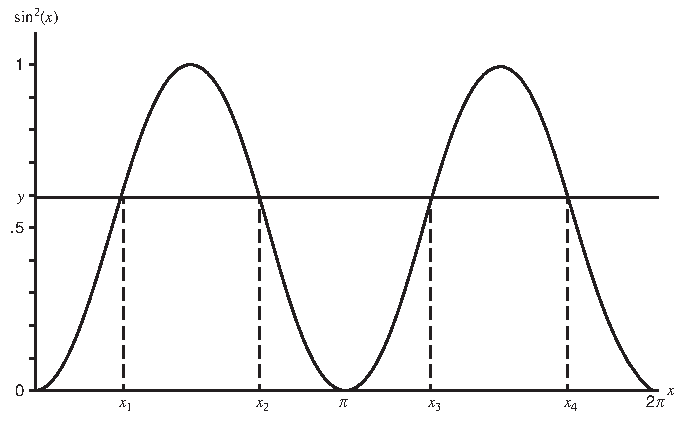
\includegraphics[width=.8\textwidth]{assets/chapter2/fig2-1-1.pdf}
\caption{\autoref{ex:2.1.2}中变换 $y=\sin^2(x)$ 的图形.}\label{fig:2.1.1}
\end{figure}
由图形的对称性和均匀分布可知，$P(X\le x_1)=P(X\ge x_4)$，而 $P(x_2\le X\le x_3)=2P(x_2\le X\le\pi)$. 因此，\eqref{eq:2.1.5}化为
\begin{equation}\label{eq:2.1.6}
P(Y\le y)=2P(X\le x_1)+2P(x_2\le X\le\pi),
\end{equation}
其中 $x_1$ 和 $x_2$ 是方程 $\sin^2x=y$ 在 $0<x<\pi$ 内的两个解. 虽然这个例子看起来很简单，所得的累积分布函数却并不简单.
\end{example}

为了避免混淆，必须留意 $X$ 和 $Y$ 的取值集合. 我们记
\begin{equation}\label{eq:2.1.7}
\mathscr X=\{x:f_X(x)>0\},\qquad
\mathscr Y=\{y:y=g(x),\ \text{其中某个 }x\in\mathscr X\}.
\end{equation}
集合 $\mathscr X$ 称为 $f_X$ 的支撑集（support set）\index{SI1015@支持集}\semanticindexanchor{1015:71}，或非正式地称为支撑（support）. 也就是说，$f_X$ 在支撑集上为正，在其他地方为零. 概率质量函数以及任意非负函数也有支撑集.

如果函数 $g$ 满足 $u>v$ 蕴含 $g(u)>g(v)$，或者满足 $u<v$ 蕴含 $g(u)>g(v)$，就称 $g$ 为单调函数（monotone function）\index{SI1040@单调}\semanticindexanchor{1040:71}；前一种情况称为递增，后一种情况称为递减. 单调函数 $g:\mathscr X\to\mathscr Y$ 是一一且满的. 每个 $x$ 对应一个 $y$，而每个 $y$ 至多对应一个 $x$，所以它是一一的；\index{SI0729@一一变换}\semanticindexanchor{729:71}由于 $\mathscr Y$ 是 $g$ 的像，它也是满的.\index{SI0730@满射变换}\semanticindexanchor{730:71}
\sourcepageanchor{72}
因此，单调函数 $g$ 把 $x$ 与 $y$ 唯一配对，$g^{-1}$ 是单值函数，并且 $g^{-1}(y)=x$ 当且仅当 $y=g(x)$.

如果 $g$ 递增，那么
\begin{equation}\label{eq:2.1.8}
\begin{aligned}
\{x\in\mathscr X:g(x)\le y\}
&=\{x\in\mathscr X:g^{-1}(g(x))\le g^{-1}(y)\}\\
&=\{x\in\mathscr X:x\le g^{-1}(y)\}.
\end{aligned}
\end{equation}
同样，如果 $g$ 递减，那么
\begin{equation}\label{eq:2.1.9}
\begin{aligned}
\{x\in\mathscr X:g(x)\le y\}
&=\{x\in\mathscr X:g^{-1}(g(x))\ge g^{-1}(y)\}\\
&=\{x\in\mathscr X:x\ge g^{-1}(y)\}.
\end{aligned}
\end{equation}
画图就能看清，为什么递减变换会使不等号反向.

如果 $g$ 递增，结合\eqref{eq:2.1.4}和\eqref{eq:2.1.8}，得到
$$F_Y(y)=\int_{\{x\in\mathscr X:x\le g^{-1}(y)\}}f_X(x)\,dx
=\int_{-\infty}^{g^{-1}(y)}f_X(x)\,dx=F_X(g^{-1}(y)).$$
如果 $g$ 递减，则
$$F_Y(y)=\int_{g^{-1}(y)}^\infty f_X(x)\,dx=1-F_X(g^{-1}(y)),$$
其中最后一步用到了 $X$ 的连续性. 这些结果可以总结如下.

\begin{theorem}\label{thm:2.1.3}\index{SI0241@单调变换}
设 $X$ 的累积分布函数为 $F_X(x)$，$Y=g(X)$，并按\eqref{eq:2.1.7}定义 $\mathscr X$ 与 $\mathscr Y$.
\begin{enumerate}
\item[(a)] 如果 $g$ 在 $\mathscr X$ 上递增，则 $F_Y(y)=F_X(g^{-1}(y))$，$y\in\mathscr Y$.
\item[(b)] 如果 $g$ 在 $\mathscr X$ 上递减且 $X$ 是连续随机变量，则 $F_Y(y)=1-F_X(g^{-1}(y))$，$y\in\mathscr Y$.
\end{enumerate}
\end{theorem}

\begin{example}[均匀分布与指数分布的关系——I]\label{ex:2.1.4}\index{SI0296@与均匀的关系}\index{SI0390@与指数的关系}
设 $X$ 在 $(0,1)$ 上服从均匀分布，概率密度函数为 $f_X(x)=1$，$0<x<1$，在其他地方为 $0$，所以 $F_X(x)=x$，$0<x<1$. 考虑随机变量 $Y=-\log X$. 因为
$$\frac d{dx}g(x)=\frac d{dx}(-\log x)=-\frac1x<0,\qquad 0<x<1,$$
$g$ 在 $\mathscr X$ 上递减. 当 $X$ 在 $0$ 与 $1$ 之间变化时，$-\log x$ 在 $0$ 与 $\infty$ 之间变化，即 $\mathscr Y=(0,\infty)$. 对 $y>0$，由 $y=-\log x$ 得 $x=e^{-y}$，所以逆函数为 $g^{-1}(y)=e^{-y}$. 因此，对 $y>0$，
$$F_Y(y)=1-F_X(g^{-1}(y))=1-F_X(e^{-y})=1-e^{-y},$$
因为 $F_X(x)=x$. 对 $y\le0$，$F_Y(y)=0$. 注意，只要求 $g$ 在 $X$ 的支撑集 $(0,1)$ 上单调即可.
\end{example}

如果 $Y$ 有连续的概率密度函数，对它的累积分布函数求导便得到该密度.
\begin{theorem}\label{thm:2.1.5}\index{SI0835@单调变换}
设 $X$ 的概率密度函数为 $f_X(x)$，$Y=g(X)$，其中 $g$ 是单调函数，$\mathscr X$ 和 $\mathscr Y$ 按\eqref{eq:2.1.7}定义. 假定 $f_X$ 在 $\mathscr X$ 上连续，$g^{-1}$ 在 $\mathscr Y$ 上有连续导数，则
\begin{equation}\label{eq:2.1.10}
f_Y(y)=\begin{cases}
f_X(g^{-1}(y))\left|\dfrac d{dy}g^{-1}(y)\right|,&y\in\mathscr Y,\\
0,&\text{其他}.
\end{cases}
\end{equation}
\end{theorem}
\sourcepageanchor{73}
\begin{proof}
由\autoref{thm:2.1.3}和链式法则，
$$f_Y(y)=\frac d{dy}F_Y(y)=\begin{cases}
f_X(g^{-1}(y))\dfrac d{dy}g^{-1}(y),&g\text{ 递增},\\
-f_X(g^{-1}(y))\dfrac d{dy}g^{-1}(y),&g\text{ 递减},
\end{cases}$$
这可以简写为\eqref{eq:2.1.10}.
\end{proof}

\begin{example}[逆伽马概率密度函数]\label{ex:2.1.6}\index{SI0313@与逆伽马的关系}\index{SI0326@与伽马的关系}
设 $f_X(x)$ 是伽马概率密度函数（gamma pdf）
$$f(x)=\frac1{(n-1)!\beta^n}x^{n-1}e^{-x/\beta},\qquad0<x<\infty,$$
其中 $\beta$ 为正常数，$n$ 为正整数. 假设我们要计算 $g(X)=1/X$ 的概率密度函数. 注意，这里支撑集 $\mathscr X$ 和 $\mathscr Y$ 都是区间 $(0,\infty)$. 若令 $y=g(x)$，则 $g^{-1}(y)=1/y$ 且 $\frac d{dy}g^{-1}(y)=-1/y^2$. 应用上述定理，对 $y\in(0,\infty)$，
$$\begin{aligned}
f_Y(y)&=f_X(g^{-1}(y))\left|\frac d{dy}g^{-1}(y)\right|\\
&=\frac1{(n-1)!\beta^n}\left(\frac1y\right)^{n-1}e^{-1/(\beta y)}\frac1{y^2}\\
&=\frac1{(n-1)!\beta^n}\left(\frac1y\right)^{n+1}e^{-1/(\beta y)},
\end{aligned}$$
这是称为逆伽马概率密度函数（inverted gamma pdf）的密度的一种特殊情形.
\end{example}

在许多应用中，函数 $g$ 可能既不递增也不递减，因而不能应用上述结果. 不过，$g$ 常常在某些区间上单调，这就使我们能够得到 $Y=g(X)$ 的分布表达式. （如果 $g$ 在任何区间上都不单调，我们就有大麻烦了.）

\begin{example}[平方变换]\label{ex:2.1.7}
设 $X$ 是连续随机变量. 对 $y>0$，$Y=X^2$ 的累积分布函数为
$$F_Y(y)=P(Y\le y)=P(X^2\le y)=P(-\sqrt y\le X\le\sqrt y).$$
由于 $X$ 连续，可以去掉左端点的等号，得到
$$\begin{aligned}
F_Y(y)&=P(-\sqrt y<X\le\sqrt y)\\
&=P(X\le\sqrt y)-P(X\le-\sqrt y)=F_X(\sqrt y)-F_X(-\sqrt y).
\end{aligned}$$
对累积分布函数求导便得到 $Y$ 的概率密度函数：
$$\begin{aligned}
f_Y(y)&=\frac d{dy}F_Y(y)\\
&=\frac d{dy}[F_X(\sqrt y)-F_X(-\sqrt y)]\\
&=\frac1{2\sqrt y}f_X(\sqrt y)+\frac1{2\sqrt y}f_X(-\sqrt y),
\end{aligned}$$
其中对 $F_X(\sqrt y)$ 和 $F_X(-\sqrt y)$ 使用了链式法则. 因此，概率密度函数为
\begin{equation}\label{eq:2.1.11}
f_Y(y)=\frac1{2\sqrt y}\bigl(f_X(\sqrt y)+f_X(-\sqrt y)\bigr).
\end{equation}
注意，\eqref{eq:2.1.11}把 $Y$ 的密度表示成两部分之和，分别对应 $g(x)=x^2$ 单调的两个区间. 一般情形也是如此.
\end{example}

\sourcepageanchor{74}
\begin{theorem}\label{thm:2.1.8}\index{SI0837@分段单调变换}
设 $X$ 的概率密度函数为 $f_X(x)$，$Y=g(X)$，并按\eqref{eq:2.1.7}定义样本空间 $\mathscr X$. 假定存在 $\mathscr X$ 的划分 $A_0,A_1,\ldots,A_k$，使得 $P(X\in A_0)=0$，且 $f_X(x)$ 在每个 $A_i$ 上连续. 再假定存在分别定义在 $A_1,\ldots,A_k$ 上的函数 $g_1(x),\ldots,g_k(x)$，满足
\begin{enumerate}
\item[(i)] 对 $x\in A_i$，$g(x)=g_i(x)$；
\item[(ii)] $g_i(x)$ 在 $A_i$ 上单调；
\item[(iii)] 对所有 $i=1,\ldots,k$，集合 $\mathscr Y=\{y:y=g_i(x),\ \text{其中某个 }x\in A_i\}$ 都相同；
\item[(iv)] 对每个 $i=1,\ldots,k$，$g_i^{-1}(y)$ 在 $\mathscr Y$ 上有连续导数.
\end{enumerate}
则
$$f_Y(y)=\begin{cases}
\displaystyle\sum_{i=1}^k f_X(g_i^{-1}(y))\left|\dfrac d{dy}g_i^{-1}(y)\right|,&y\in\mathscr Y,\\
0,&\text{其他}.
\end{cases}$$
\end{theorem}

\autoref{thm:2.1.8}的关键在于，可以把 $\mathscr X$ 分成集合 $A_1,\ldots,A_k$，使 $g(x)$ 在每个 $A_i$ 上单调. 因为 $P(X\in A_0)=0$，我们可以忽略这个“例外集”$A_0$. 这是一种技术处理，例如可用于处理区间端点. 要注意，每个 $g_i(x)$ 都是一一地把 $A_i$ 映到整个 $\mathscr Y$ 的变换. 此外，$g_i^{-1}(y)$ 是从 $\mathscr Y$ 到整个 $A_i$ 的一一函数；对 $y\in\mathscr Y$，$g_i^{-1}(y)$ 给出唯一的 $x=g_i^{-1}(y)\in A_i$，使得 $g_i(x)=y$. （推广见\autoref{exercise:2.7}.）

\begin{example}[正态分布与卡方分布的关系]\label{ex:2.1.9}\index{SI0284@与正态的关系}\index{SI0366@与卡方的关系}
设 $X$ 具有标准正态分布（standard normal distribution），
$$f_X(x)=\frac1{\sqrt{2\pi}}e^{-x^2/2},\qquad-\infty<x<\infty.$$
考虑 $Y=X^2$. 函数 $g(x)=x^2$ 在 $(-\infty,0)$ 和 $(0,\infty)$ 上单调，集合 $\mathscr Y=(0,\infty)$. 应用\autoref{thm:2.1.8}，取
$$\begin{aligned}
A_0&=\{0\};\\
A_1&=(-\infty,0),&g_1(x)&=x^2,&g_1^{-1}(y)&=-\sqrt y;\\
A_2&=(0,\infty),&g_2(x)&=x^2,&g_2^{-1}(y)&=\sqrt y.
\end{aligned}$$
$Y$ 的概率密度函数为
$$\begin{aligned}
f_Y(y)&=\frac1{\sqrt{2\pi}}e^{-(-\sqrt y)^2/2}\left|-\frac1{2\sqrt y}\right|
+\frac1{\sqrt{2\pi}}e^{-(\sqrt y)^2/2}\left|\frac1{2\sqrt y}\right|\\
&=\frac1{\sqrt{2\pi}}\frac1{\sqrt y}e^{-y/2},\qquad0<y<\infty.
\end{aligned}$$
这是我们将经常遇到的密度，即自由度为 $1$ 的卡方随机变量（chi squared random variable）的概率密度函数.
\end{example}

本节最后介绍一种特殊而又非常有用的变换.
\begin{theorem}[概率积分变换]\label{thm:2.1.10}\index{SI0847@概率积分变换}
设 $X$ 具有连续的累积分布函数 $F_X(x)$，并定义随机变量 $Y=F_X(X)$. 则 $Y$ 在 $(0,1)$ 上服从均匀分布，即 $P(Y\le y)=y$，$0<y<1$.
\end{theorem}
在证明这个定理之前，我们暂且岔开，详细考察 $F_X^{-1}$，也就是累积分布函数 $F_X$ 的逆. 如果 $F_X$ 严格递增，则可用下式良好地定义 $F_X^{-1}$：
\begin{equation}\label{eq:2.1.12}
F_X^{-1}(y)=x\quad\Longleftrightarrow\quad F_X(x)=y.
\end{equation}
\sourcepageanchor{75}
\begin{figure}[htbp]\centering
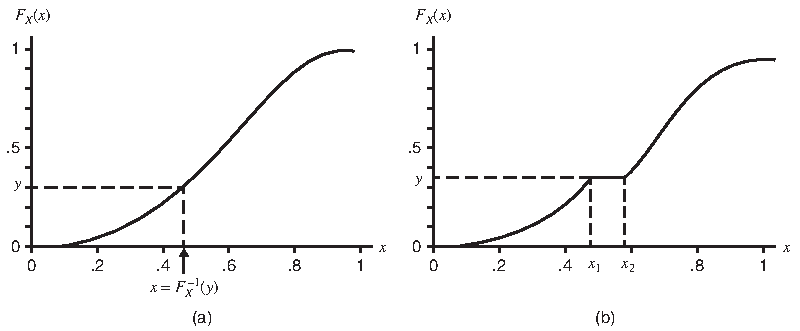
\includegraphics[width=\textwidth]{assets/chapter2/fig2-1-2.pdf}
\caption{(a) $F(x)$ 严格递增；(b) $F(x)$ 非递减.}\label{fig:2.1.2}
\end{figure}
然而，如果 $F_X$ 在某个区间上为常数，\eqref{eq:2.1.12}就不能良好地定义 $F_X^{-1}$，如\autoref{fig:2.1.2}所示. 任意满足 $x_1\le x\le x_2$ 的 $x$ 都满足 $F_X(x)=y$.

为避免这一问题，对 $0<y<1$，定义
\begin{equation}\label{eq:2.1.13}
F_X^{-1}(y)=\inf\{x:F_X(x)\ge y\}.
\end{equation}
当 $F_X$ 不为常数时，这一定义与\eqref{eq:2.1.12}一致；即使 $F_X$ 并非严格递增，它也给出了单值的 $F_X^{-1}$. 使用这一定义，\autoref{fig:2.1.2}(b) 中有 $F_X^{-1}(y)=x_1$. 在 $y$ 的取值范围的端点，也可以定义 $F_X^{-1}(y)$：如果对所有 $x$ 都有 $F_X(x)<1$，则 $F_X^{-1}(1)=\infty$；对任意 $F_X$，均有 $F_X^{-1}(0)=-\infty$.

\begin{proof}[\autoref{thm:2.1.10}的证明]
对于 $Y=F_X(X)$，当 $0<y<1$ 时，
$$\begin{aligned}
P(Y\le y)&=P(F_X(X)\le y)\\
&=P(F_X^{-1}[F_X(X)]\le F_X^{-1}(y))&&\text{（$F_X^{-1}$ 递增）}\\
&=P(X\le F_X^{-1}(y))&&\text{（见下文）}\\
&=F_X(F_X^{-1}(y))&&\text{（$F_X$ 的定义）}\\
&=y.&&\text{（$F_X$ 的连续性）}
\end{aligned}$$
在端点处，当 $y\ge1$ 时 $P(Y\le y)=1$，当 $y\le0$ 时 $P(Y\le y)=0$，这表明 $Y$ 服从均匀分布.

等式
$$P\bigl(F_X^{-1}(F_X(X))\le F_X^{-1}(y)\bigr)=P(X\le F_X^{-1}(y))$$
背后的理由略有些微妙，值得进一步说明. 如果 $F_X$ 严格递增，确实有 $F_X^{-1}(F_X(x))=x$. （参见\autoref{fig:2.1.2}(a).）然而，如果 $F_X$ 有平坦部分，就可能有 $F_X^{-1}(F_X(x))\ne x$. 假设 $F_X$ 如\autoref{fig:2.1.2}(b) 所示，且 $x\in[x_1,x_2]$，则对该区间内的任意 $x$，都有 $F_X^{-1}(F_X(x))=x_1$.
\sourcepageanchor{76}
即使如此，概率的等式仍然成立，因为对任意 $x\in[x_1,x_2]$，都有 $P(X\le x)=P(X\le x_1)$. 累积分布函数的平坦部分表示一个概率为 $0$ 的区域，即 $P(x_1<X\le x)=F_X(x)-F_X(x_1)=0$.
\end{proof}

\autoref{thm:2.1.10}的一个应用是从给定分布产生随机样本.\index{SI0861@随机数生成}\semanticindexanchor{861:76} 如果需要从累积分布函数为 $F_X$ 的总体产生一个观测值 $X$，只需在 $0$ 与 $1$ 之间产生一个均匀随机数 $U$，然后由方程 $F_X(x)=u$ 解出 $x$. （对许多分布，存在耗费更少计算时间的其他观测值生成方法；不过，本方法具有普遍适用性，因而仍然有用.）
